
\subsection{Europa}

La instancia elegida para analizar en Europa, fue la universidad Complutense de Madrid (\textit{ucm.es}), ubicada aproximadamente a
5 km de la capital de Madrid. El objetivo de ésta instancia, fue hacer un traceroute a una universidad de Europa central, para poder 
probar y analizar alguna universidad que se situe en Europa y que obligatoriamente tenga que dar el salto del Reino Unido a Europa, 
y así poder observar si hay mucha diferencia o no, en cuanto a tiempos y performance, de ese salto obligatorio de más. \\

Para éste caso, se esperaba que haya tres saltos intercontinentales. Uno de Argentina a USA, otro de USA a Inglaterra (esto lo esperabamos
porque primero hicimos el experimento de analizar una universidad en Inglaterra, no suponiamos ni sabiamos que de Estados Unidos iba a pasar
por Inglaterra) y un último salto de Ingleterra a España. Esto sucede y lo podemos observar gracias a los resultados obtenidos. \\

Los datos de la tabla a continuación, fueron el resultado de 30 iteraciones para cada TTL, hasta la universidad de Madrid: \\


\begin{tabular}{ |p{2cm}||p{3cm}|p{3cm}|p{3cm}|p{3cm}|   }
 \hline
 \multicolumn{5}{|c|}{Traceroute a Madrid, España} \\
 \hline
 \textit{TTL} & \textit{IP}  & \textit{RTT} & $\delta$\textit{RTT} & \textit{z}$\delta$\textit{RTT}\\
 \hline
 1   & Sin respuesta  & - &   - & -\\
 2   & 10.10.10.1 & 5.0 ms &   - & -\\
 3   & 190.3.128.11  & 13.97 ms & 8.97 ms & 0.79  \\
 4   & 190.3.128.34   & 13.16 ms &   - & -\\	
 5   & 64.215.24.153  & 18.03 ms &  4.87 ms & 0.88\\
 6   &  67.17.94.249 & 140.06 ms &  122.03 ms & 1.57\\
 7   & Sin respuesta  & - &  - & -\\
 8   & 4.69.210.222  & 245.33 ms & 105.27 &  1.22\\
 9   & 4.69.210.222 & 245.29 ms &  - & -\\
 10   & 213.242.113.78   & 260.68 ms & 15.39 ms & 0.66\\
 11   & 130.206.245.1   & 258.76 ms & 25.08 ms & 0.46\\
 12   & 130.206.212.106  & 275.93 ms &  - & -\\
 13   & Sin respuesta  & - & - & -\\
 14   & Sin respuesta  & - & - & -\\
 15   & Sin respuesta  & - & - & -\\
 16   & Sin respuesta  & - & - & -\\
 17   & Sin respuesta  & - & - & -\\
 18   & Sin respuesta  & - & - & -\\
 19   & Sin respuesta  & - & - & -\\
 20   & Sin respuesta  & - & - & -\\
 21   & Sin respuesta  & - & - & -\\
 \hline
\end{tabular}


Análisis de la tabla de RTT's: \\ \\

La primera respuesta que obtenemos es para TTL=1, la IP 10.10.10.1 se corresponde con el router Wi-Fi que se está utilizando en el hogar del 
integrante que corrió el experimento. Se corresponde con una red privada que no es visible para afuera y que utiliza protocolo IP versión 4 (IPv4). \\
Las IP's de TTL=3 y TTL=4 se corresponden con las IP's de la Cooperativa Telefonica de Telviso, proveedor de internet ubicado en 
la localidad de Del Viso, partido de Pilar (zona norte GBA). \\
La IP de TTL=5 se corresponde con un servidor de la ciudad de Denver, Colorado. Esto se dedujo buscando la ip en internet. \\






\pagebreak


\begin{figure}[!h]
\centering
\caption{Saltos vs RTT}
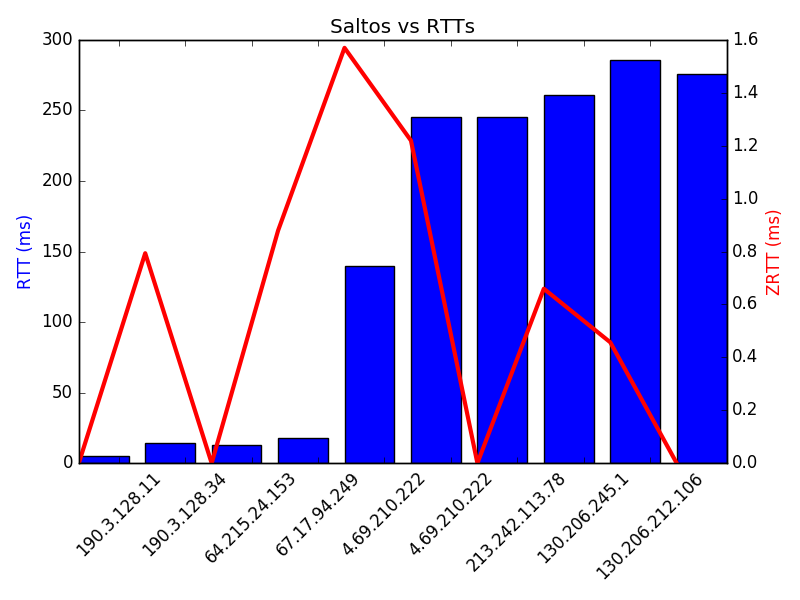
\includegraphics[width=0.75\textwidth]{modules/grafico-rtt-EU}
 \label{fig:grafico-rtt-EU}
\end{figure}

\pagebreak

\begin{figure}[!h]
\centering
\caption{traceroute de ARG a ESP}
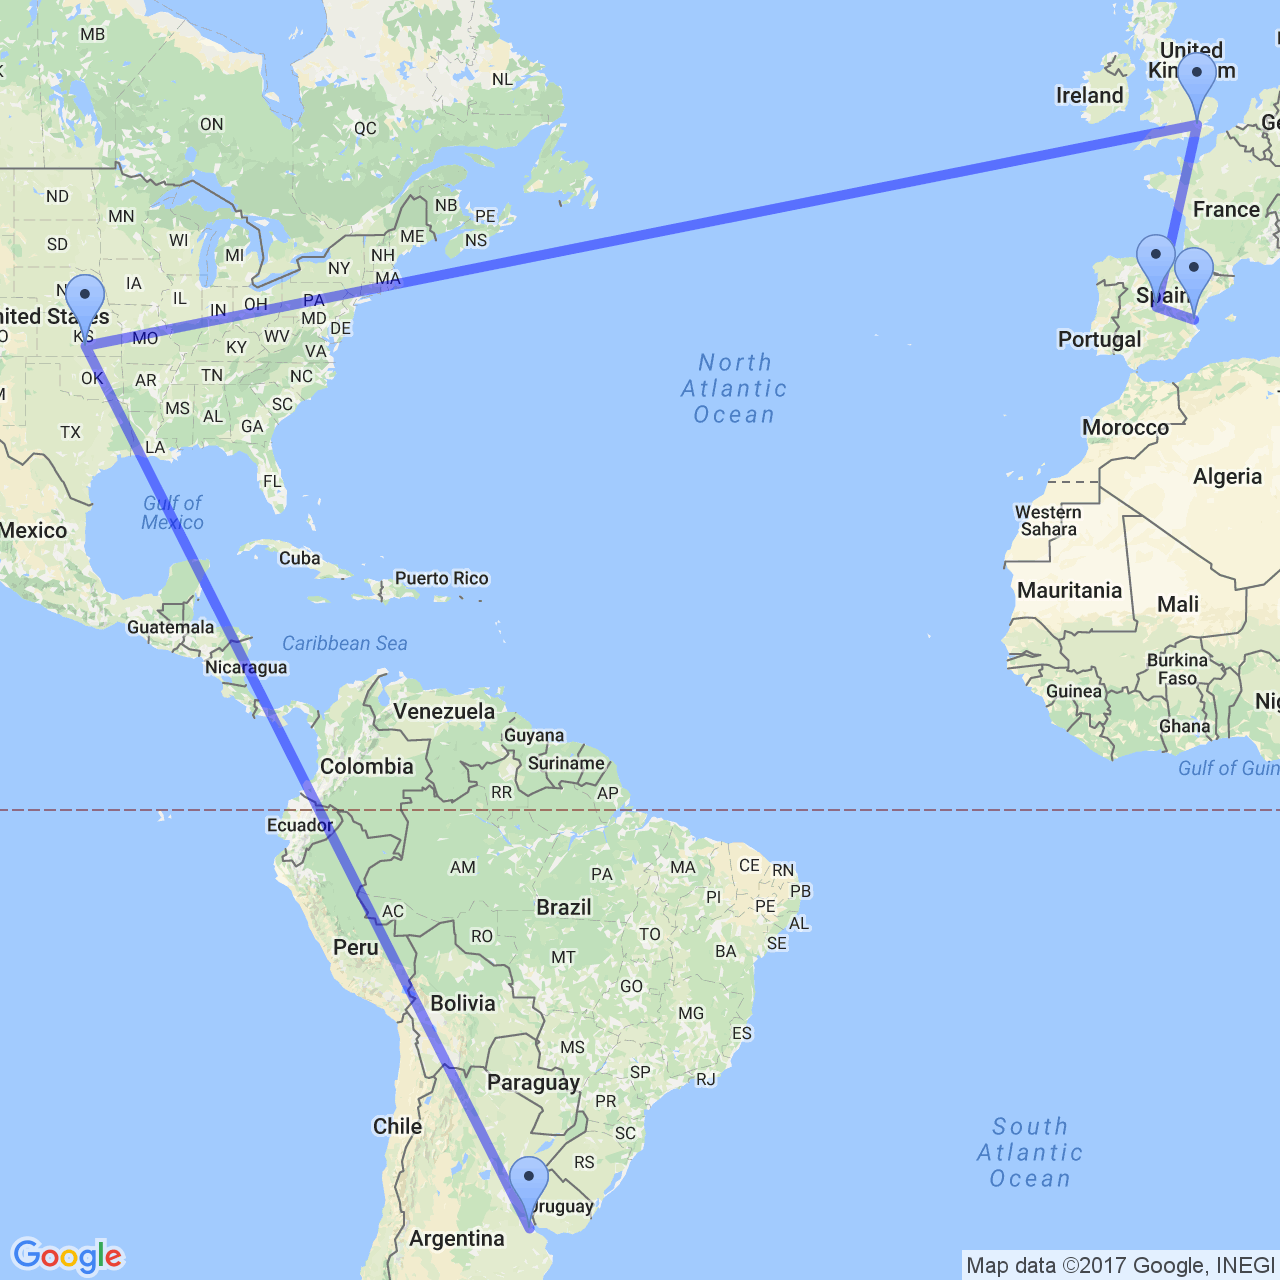
\includegraphics[width=0.75\textwidth]{modules/traceroute-EU}
 \label{fig:traceroute-EU}
\end{figure}
